\documentclass[sigconf,10pt,nonacm]{acmart}

\hfuzz=100pt
\hbadness=99999
\vbadness=99999

\renewcommand\footnotetextcopyrightpermission[1]{}

\pdfstringdefDisableCommands{%
  \def\\{}%
}

\usepackage{hyperref}
\usepackage{graphicx} 
\usepackage{listings} 

\AtBeginDocument{%
  \providecommand\BibTeX{{%
    Bib\TeX}}}

\setcopyright{acmlicensed}
\copyrightyear{2025}
\acmYear{2025}
\acmDOI{XXXXXXX.XXXXXXX}


\begin{document}

\title[TinyML Parking Vacancy Detection]{An On-Device TinyML Approach for Parking Lot Vacancy Detection}

\author{Matteo Lorenzoni}
\email{matteo.lorenzoni-1@studenti.unitn.it}

\author{Florian Remberger}
\email{florian.remberger@studenti.unitn.it}

\affiliation{%
  \institution{University of Trento}
  \streetaddress{Via Sommarive 9}
  \city{Povo}
  \state{Trento}
  \country{Italy}
  \postcode{38123}
}

\renewcommand{\shortauthors}{Lorenzoni and Remberger}


\begin{abstract}
The increasing urbanization and vehicle density in cities make finding an available parking space a significant challenge, leading to traffic congestion and increased emissions. While many solutions exist, they often rely on expensive sensors or powerful, cloud-connected processing units. This paper presents a low-cost, low-power solution for parking lot vacancy detection using Tiny Machine Learning (TinyML). Our approach pivots from complex object detection models to a lightweight binary image classifier deployed on a highly resource-constrained microcontroller, the ARDUINO Nano 33 BLE Sense Lite. The system processes an image from a fixed camera, crops individual parking spaces using predefined coordinates, and classifies each space as 'occupied' or 'empty'. Our implemented Convolutional Neural Network (CNN) achieves a validation accuracy of 99.40\% and performs inference in approximately 120ms per slot on the target hardware. This work demonstrates the feasibility of deploying accurate computer vision models on minimal hardware, offering a scalable and energy-efficient alternative for smart parking systems.
\end{abstract}

\maketitle

\section{Motivation}
\label{sec:motivation}
Finding a parking space in urban centers is a common source of frustration for drivers, contributing significantly to traffic congestion, wasted fuel, and increased carbon emissions. Studies have shown that a substantial portion of urban traffic is composed of vehicles "cruising" for parking. This inefficiency highlights a clear need for intelligent systems that can provide real-time information about parking availability. An effective smart parking solution can guide drivers directly to empty spots, saving time, reducing stress, and mitigating the environmental impact of unnecessary driving.

The problem this work attacks is the development of an \textbf{accessible, low-cost, and low-power parking vacancy detection system}. While camera-based solutions are common, they often require significant computational power, either on-site with expensive edge computers (like NVIDIA Jetson) or via a constant, high-bandwidth connection to a cloud server for processing. These requirements create a high barrier to entry in terms of cost and infrastructure. Our goal is to leverage the advancements in Tiny Machine Learning (TinyML) to bring the required intelligence directly onto a small, affordable microcontroller, thus creating a self-contained and highly efficient system.

\section{Limitations of the State of the Art}
\label{sec:limitations}
The state of the art in parking occupancy detection can be broadly categorized into sensor-based and vision-based systems.

\noindent\textbf{Sensor-based systems} typically use ultrasonic, infrared, or magnetic sensors embedded in each parking space. While accurate, this approach suffers from high installation and maintenance costs, making it difficult to scale across large parking lots or entire city streets.

\noindent\textbf{Vision-based systems} use cameras to monitor multiple parking spaces at once, making them more cost-effective per slot. The primary challenge lies in processing the visual data. High-end approaches utilize complex Deep Learning models like You Only Look Once (YOLO) or Faster R-CNN for vehicle detection. These models provide excellent accuracy but are computationally demanding, requiring powerful GPUs for real-time processing, which is often done in the cloud. This reliance on the cloud introduces latency, privacy concerns, and a dependency on network connectivity.

Recent efforts have aimed to bring vision processing to the edge to mitigate these issues. Some research explores deploying CNNs on more capable single-board computers like the Raspberry Pi \cite{rpi-parking}. However, these devices still consume significantly more power and are more expensive than microcontrollers. The true frontier of TinyML is to enable such applications on devices with memory measured in kilobytes, not gigabytes. The literature shows that deploying even simplified CNNs on microcontrollers for vision tasks is a significant challenge due to extreme memory (RAM and Flash) constraints \cite{tinyml-challenges}. Our work addresses this specific gap by designing a system explicitly for such a highly constrained environment.

\section{Key Insights}
\label{sec:key-insights}
The primary obstacle we faced was the memory limitation of our target hardware, the ARDUINO Nano 33 BLE Sense Lite, which has only 256KB of RAM and 1MB of Flash memory. Our initial attempt to train and deploy a quantized YOLOv11n model for object detection failed, as the model was still too large to fit within these constraints. This led to the key insight of this project:

\noindent\textbf{Architectural Pivot from Detection to Classification.} Instead of using a single, complex model to find all cars in a large image, we changed the problem definition. We simplified the task from object detection to binary image classification. This insight has two main components:
\begin{enumerate}
    \item \textbf{Problem Decomposition:} The system leverages a fixed camera perspective. By knowing the exact bounding box coordinates of each parking slot beforehand, we can programmatically crop the main image into a series of smaller images, one for each slot.
    \item \textbf{Simplified Model:} We then only need to solve a much simpler problem: classifying each small image as either `occupied` or `empty`. A binary classifier is significantly smaller and less computationally intensive than a multi-object detection model.
\end{enumerate}

This architectural shift is what makes our approach effective and novel for this hardware class. It advances the state of the art by providing a practical methodology to circumvent the primary limitation—model size—that prevents complex vision tasks from being deployed on low-cost microcontrollers. It is more effective than past approaches for this specific context because it trades the generality of object detection for the extreme efficiency of binary classification, which is a perfect fit for a dedicated, single-purpose device.

\section{Main Artifacts}
\label{sec:main-artifacts}
The main artifact of this project is a complete, end-to-end software system for parking vacancy detection designed for and deployed on a microcontroller. These artifacts include:
\begin{itemize}
    \item A Python script for preprocessing images and generating labeled datasets.
    \item A lightweight Convolutional Neural Network (CNN) model trained to classify parking slots as `occupied` or `empty` as tflite model.
    \item An Arduino sketch that runs the trained model on the ARDUINO Nano 33 BLE Sense Lite, performing inference on images of parking slots by cropping them from a larger image and classifying each slot.
\end{itemize}

\noindent\textbf{Methodology and Implementation}

The system's workflow is as follows:
\begin{enumerate}
    \item An grayscale, 160x120 image of a parking lot is captured via the OV7675 camera module. 
    \item Predefined bounding box coordinates are used to crop the main image into multiple smaller images, each containing exactly one parking slot.
    \item Each cropped image is resized to the model's input dimensions and fed into the classification model.
    \item The model performs inference and outputs a classification (`occupied` or `empty`) for each slot.
\end{enumerate}

\noindent\textbf{Dataset Preparation:} We used the PKLot dataset \cite{pklot}, which contains images of parking lots with annotated bounding boxes for each car. A significant part of our work involved writing scripts to process this dataset. Since our model needed to classify empty slots as well, we had to modify the dataset to generate labeled images for both `occupied` and `empty` states. This data preparation was a time-consuming but crucial step to create a suitable training set for our classification approach.

\noindent\textbf{Hardware:} The core of our system is the \textbf{ARDUINO Nano 33 BLE Sense Lite}. Its Arm® Cortex®-M4F processor, running at 64 MHz, is capable of running optimized machine learning models using frameworks like TensorFlow Lite for Microcontrollers. Its extremely limited memory (256KB RAM, 1MB Flash) was the driving constraint for our design choices.

\noindent\textbf{Model Architecture and Training:} Our final artifact is a lightweight Convolutional Neural Network (CNN). The architecture was designed to have a minimal number of parameters while still being effective for the task.
The model consists of two convolutional blocks followed by a dense layer, as detailed below:
\begin{verbatim}
Model: "sequential"
____________________________________________________
 Layer (type)                Output Shape          
====================================================
 rescaling (Rescaling)       (None, 48, 48, 1)     
                                                 
 conv2d (Conv2D)             (None, 46, 46, 8)     
                                                 
 max_pooling2d (MaxPooling2D) (None, 23, 23, 8)     
                                                 
 conv2d_1 (Conv2D)           (None, 21, 21, 16)    
                                                 
 max_pooling2d_1 (MaxPooling2D) (None, 10, 10, 16)    
                                                 
 flatten (Flatten)           (None, 1600)          
                                                 
 dense (Dense)               (None, 16)            
                                                 
 dense_1 (Dense)             (None, 1)             
====================================================
\end{verbatim}
The model was trained for just \textbf{5 epochs} using the \textbf{Adam optimizer}. It was then converted to a TensorFlow Lite model and quantized to 8-bit integers (INT8) to further reduce its size and make it compatible with the Arduino's processor.

\noindent\textbf{Evaluation:} The artifact was evaluated on two key metrics: classification accuracy and on-device performance. The model's accuracy was assessed using a validation set, and its real-world performance was measured by timing the inference process directly on the Arduino hardware.

\section{Key Results and Contributions}
\label{sec:key-contributions}
Our approach yielded highly successful results, demonstrating that TinyML can be effectively applied to this practical computer vision problem.

\begin{figure}[h!]
  \centering
  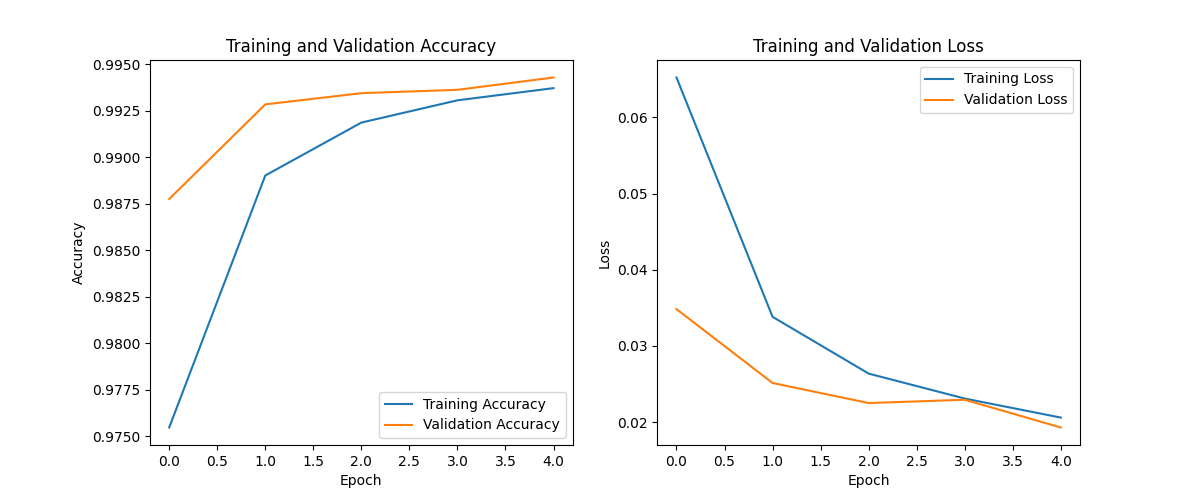
\includegraphics[width=\linewidth]{./images/training_results.png}
  \caption{Training and validation accuracy/loss curves over 5 epochs. The stable validation accuracy (top) and low validation loss (bottom) demonstrate the model's effective learning without overfitting.}
  \label{fig:training_results}
\end{figure}

\noindent\textbf{Key Empirical Results:}
\begin{enumerate}
    \item \textbf{High Classification Accuracy:} The model achieved a \textbf{validation accuracy of 99.40\%} and a training accuracy of 99.25\%. This outstanding result shows that the simplified classification model can distinguish between occupied and empty parking slots with a very high degree of reliability.
    \item \textbf{Efficient On-Device Performance:} When deployed on the ARDUINO Nano 33 BLE Sense Lite, the quantized model performed inference on a single parking slot image in approximately \textbf{120-121 milliseconds}. This swift performance allows a system to scan a multi-slot parking lot in a matter of seconds, making it suitable for real-time applications.
\end{enumerate}

\noindent\textbf{Contributions:}
This paper makes the following contributions to the field of low-power embedded systems and TinyML:
\begin{itemize}
    \item \textbf{A validated architectural pivot for resource-constrained vision tasks.} We demonstrated that by decomposing a complex object detection problem into a series of simpler binary classifications, it is possible to achieve the desired outcome on hardware that would otherwise be unsuitable. This methodology serves as a practical template for other TinyML projects facing similar memory constraints.
    
    \item \textbf{An open-source, end-to-end system for parking detection on an Arduino-class microcontroller.} We provide the full implementation, from data preparation to model training and on-device deployment. This serves as a concrete example that bridges the gap between theoretical TinyML concepts and practical, real-world application.
    
    \item \textbf{Quantitative performance benchmarks for a CNN on the ARDUINO Nano 33 BLE Sense Lite.} Our reported results for accuracy and inference time provide valuable data points for other researchers and developers working with this popular microcontroller, helping them gauge the feasibility and potential performance of their own projects.
\end{itemize}

Our work successfully overcomes the limitations of both expensive sensor-based systems and power-hungry vision systems by creating a solution that is low-cost, highly accurate, and energy-efficient.

\begin{thebibliography}{9}

\bibitem{pklot}
Almeida, Patrick and Oliveira, Luiz S. and Silva Jr, E. and Britto Jr, A. and Koerich, A. (2015).
PKLot--A robust dataset for parking lot classification.
\textit{2015 International Joint Conference on Neural Networks (IJCNN)}.

\bibitem{rpi-parking}
Amato, G., Carrara, F., Falchi, F., Gennaro, C., Meghini, C., \& Vairo, C. (2017).
Car Parking Occupancy Detection Using Smart Camera Networks and Deep Learning.
\textit{2017 14th IEEE International Conference on Advanced Video and Signal Based Surveillance (AVSS)}.

\bibitem{tinyml-challenges}
Banbury, C., Reddi, V. J., \& Sze, V. (2021).
Tiny Machine Learning: Progress and Futures.
\textit{arXiv preprint arXiv:2403.19076}.

\end{thebibliography}

\end{document}
